\chapter{Część teoretyczna}\label{chap:teoria}
Ten rozdział powinien zawierać teorię z~której autor będzie korzystał w~dalszej
części pracy.  Podstawowym celem istnieniem tego rozdziału jest umożliwienie
czytelnikowi zrozumienie teorii rozwijanej w pracy oraz osiągniętych wyników
praktycznych.  Jeżeli jakieś informacje nie są niezbędne do zrozumienia
osiągnięć autora nie należy o nich pisać.

\section{Architektura Glasgow Haskell Compiler}

\begin{figure}[ht]
    \centering
    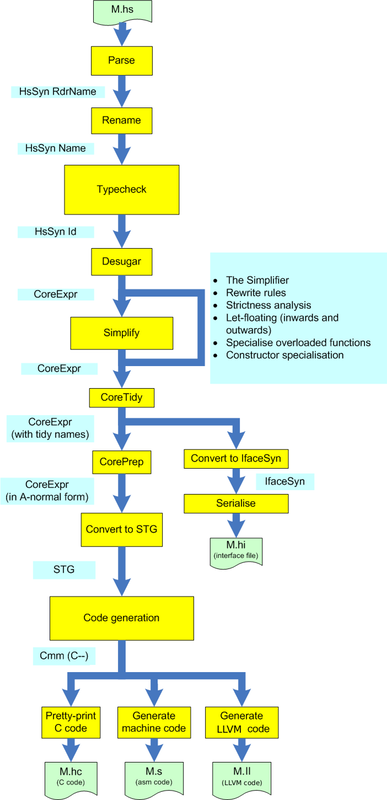
\includegraphics[width=0.8\textwidth]{images/AOSA_compiler}
    \caption{Schemat Glasgow Haskell Compiler\cite{AOSA}}
    \label{fig:AOSA_compiler}
\end{figure}

\todo[inline]{Treść. Rysunek z AOSA. Frontend i backed. Opis parser, renamer, type-checker.}

\sectionex{Rodziny typów}{Rozszerzenie TypeFamilies}
\todo[inline]{Treść zaczerpnięta z UsersGuide. Pamiętać o DataFamilies}

\sectionex{Częściowe sygnatury typów}{Rozszerzenie PartialTypeSignatures}
\todo[inline]{Treść zaczerpnięta z UsersGuide. Pamiętać o NamedWildCards}
